\documentclass{article}

\usepackage{arxiv}
\usepackage{amsmath, amsfonts, amssymb}
\usepackage{graphicx}
\usepackage{hyperref}
\usepackage{booktabs}
\usepackage{float}
\usepackage{tikz}
\usetikzlibrary{arrows.meta, positioning, shapes.geometric}
\setlength{\headheight}{23pt}
\makeatletter
\def\headeright{}
\def\undertitle{}
\makeatother
\AtBeginDocument{
  \setlength{\headheight}{23pt}
  \addtolength{\topmargin}{-9pt}
}

\title{Intermediate Artifacts as First-Class Citizens:\\
A Data Model for Durable Intermediate Artifacts in Agentic Systems}

\author{
  Josh Rosen \\
  ThruWire, Inc.
  \And
  Seth Rosen \\
  ThruWire, Inc.
}

\begin{document}

\maketitle

\begin{abstract}
Many contemporary AI systems are organized around iterative loops in which models reason, call tools, observe results, and continue until a task is complete. These systems often produce final artifacts such as memos, plans, recommendations, and analyses, while the intermediate work that shaped those outputs remains ephemeral. This paper argues that the final artifact is the wrong durable state boundary. Final artifacts are lossy projections over upstream state: evidence selections, claim structures, criteria, plans, transformations, assumptions, and methods of synthesis. Important intermediate work may help produce a good result on a given run, yet still disappear before later humans or agents can inspect it, reuse it, or improve it.

We argue that selected intermediate outputs should therefore be treated as first-class artifacts: typed, structured, addressable, versioned, dependency-aware, authoritative, and consumable by downstream computation. Some of these artifacts are published reasoning structures, such as decompositions, assumptions, evidence mappings, decision procedures, transformation rules, and reconstruction methods; others are planning, evidence, transformation, or synthesis artifacts. In all cases, they provide durable state boundaries for inspection, revision, reuse, and downstream consumption. Only inspectable intermediate artifacts make it possible to improve final artifacts durably across iterative, long-horizon work; only lineage over those artifacts makes it possible to trace logic errors, incorrect assumptions, or false information back to the source where they entered the system.

The contribution is a systems-level data model. We distinguish intermediate artifacts from transcripts, memory, hidden chain-of-thought, and final answers; formalize additive and superseding update semantics with explicit current-state resolution; and describe how artifact lineage supports maintained artifact state and longitudinal improvability across runs, agents, and revisions. Without such state, final artifacts become opaque revision targets: they can be patched, but not reliably corrected at the source, which increases the risk of drift and hidden correctness failures over time.
\end{abstract}

\section{Introduction}

Many current AI systems are organized around iterative loops in which a model reasons, calls tools, observes results, and continues until it decides it is done. Such loops are powerful for one-off tasks. The central systems question for revisable work, however, is not only whether a model can produce a plausible answer now. It is whether the surrounding system preserves the state needed to inspect, diagnose, revise, and extend that work later.

Most current LLM interfaces still privilege final answers. Some systems expose narrated thinking or chain-of-thought-like text that users can see, even though such narration may be post hoc or otherwise unfaithful to the model's internal process. Other intermediate state may exist only in hidden model computation, controller state inside the harness, or accumulated chat history and transcript context. None of these surfaces is a reliable durable state boundary. Hidden state is not directly inspectable. Surfaced narration and chat history may be readable, but they are usually not preserved as typed, editable, authoritative intermediate objects that later work can consume directly. As a result, the parts of the process that most directly shaped a result often disappear after execution or remain visible only in weak, transcript-shaped form.

A multi-step process that produces an evidence digest, claim matrix, criteria artifact, plan, and final memo is not well modeled as one prompt plus one answer. That intermediate work may be useful, careful, and even task-helpful on the run that produced it. The problem is not that such work is bad. The problem is that if it remains ephemeral, later work cannot inspect it, build on it, or improve it coherently.

Intermediate artifacts provide durable state at these decomposition boundaries. They preserve the evidence selections, decompositions, criteria, plans, transformations, and partial products from which later work should proceed. A final artifact is a lossy projection over those upstream choices, which means that once intermediate state is flattened into final prose, later improvement often requires reconstruction rather than inspection. If final artifacts are to improve durably over long-horizon work, the intermediate artifacts that shaped them must remain inspectable and editable.

Intermediate artifacts are not the model's private chain-of-thought. They are durable maintained state. Some encode published reasoning structures: explicit decompositions, assumptions, evidence mappings, criteria, decision procedures, transformation rules, and reconstruction methods that the system chooses to preserve. The purpose is not to expose hidden reasoning traces, but to maintain intermediate structures that later work can inspect, revise, and reuse.

This matters because a system that preserves intermediate artifacts exposes more durable loci of intervention than one that repeatedly revises only the final rendered output. It also makes error resolution source-directed rather than cosmetic: if a conclusion is wrong because of a false premise, a stale evidence digest, or a flawed decision rule, lineage over intermediate artifacts makes it possible to locate where that problem entered the work and correct it there.

Prior work introduced \emph{execution lineage} as an execution model for AI-native work represented as deterministic graphs of artifact-producing computation. Its central question was: \emph{how should such work execute?} The present paper addresses the complementary question: \emph{what durable state should that execution produce?} The answer we defend is that selected intermediate artifacts should be treated as first-class citizens of the system. They are not merely logs, not only UI affordances, and not simply cached prompt fragments. They are maintained state.

Although this paper often discusses reasoning-relevant artifacts, the proposed model is not limited to reasoning in the narrow sense. The same state problem appears whenever AI work is decomposed into intermediate products: evidence digests, transformations, plans, criteria, partial drafts, decision matrices, implementation steps, or synthesis procedures. The common property is not that every artifact is ``reasoning,'' but that each artifact is a durable boundary in a larger system. Treating those boundaries as first-class state makes the system inspectable, revisable, reusable, and buildable over time.

This paper is a systems position paper and conceptual data-model proposal. Its claim is that revisable LLM systems require durable intermediate state if their outputs are to remain inspectable, diagnosable, improvable, and buildable over time.

Our thesis is:
\begin{quote}
LLM systems should treat selected intermediate outputs as durable, addressable artifacts because final artifacts are lossy projections over upstream state. Improving, diagnosing, or extending a final artifact often requires access to the intermediate objects where evidence, assumptions, criteria, transformations, plans, decision procedures, reconstruction methods, or partial products were introduced.
\end{quote}

Intermediate artifacts are the editable substrate of final-artifact quality. Reasoning artifacts are one important subtype; the broader model concerns durable intermediate state at decomposition boundaries.

The paper makes four contributions. First, it formulates an artifact-centric data model for revisable LLM systems and defines the properties that make an artifact first-class, including authority and current-state resolution. Second, it distinguishes \emph{artifact lineage} from \emph{prompt lineage}, execution lineage, memory, and final outputs. Third, it introduces additive versus superseding update semantics as a mechanism for maintaining coherent intermediate state over time. Fourth, it argues that evaluating persistent systems requires attention to maintained-state quality and to the intervention surfaces preserved across revisions, not only final-output acceptability.

Our claim is deliberately narrow and system-level. We do not claim model-level determinism, nor do we claim that every task requires durable artifacts. Some short-horizon conversational tasks do not. We also do not claim that schemas or structured artifacts are free; they require discipline, publication boundaries, and explicit tradeoffs against flexibility. The claim is instead that once AI work becomes multi-step, revisable, and shared across time, persistent progress depends on intermediate artifacts that sit alongside transcripts, hidden reasoning, and final outputs as the maintainable state surface.

\section{Motivating Example}

Consider a policy-analysis system that produces a recommendation memo about telehealth expansion. A plausible execution includes source digests for utilization, reimbursement, operations, and access-cost tradeoffs; a claim matrix grounded in those sources; a tension analysis that preserves unresolved conflicts; a recommendation-criteria artifact; an implementation plan; and finally a memo.

Now suppose a year-one budget-neutrality constraint arrives after an initial draft. A weak final memo could have several distinct upstream causes. The evidence digest may have omitted budget facts. The claim matrix may have overstated access benefits relative to cost. The criteria artifact may have failed to encode year-one neutrality as a hard constraint. The tension analysis may have collapsed an access-versus-cost tradeoff too aggressively. The implementation plan may have assumed unrestricted rollout. The reconstruction procedure that synthesized the memo may have used the wrong priority order. A decision rule may have failed to distinguish hard constraints from preferences.

A transcript-centric system can rewrite the memo to mention budget neutrality, but it cannot necessarily identify which upstream object caused the weakness or preserve the parts of the prior reasoning that remain valid. The final answer does not expose the state boundary where revision should occur. Diagnostic revision means tracing an unsatisfactory final artifact back to the upstream intermediate artifact where the relevant assumption, omission, compression, or transformation entered the work.

Conversely, some of the most valuable prior work may deserve preservation. The original claim matrix may contain a useful access-equity framing. The tension analysis may preserve a valuable unresolved tradeoff. The prior plan may contain a viable phased-rollout sequence even if its recommendation logic needs revision. If those contributions exist only as transient reasoning or prose embedded in the final memo, the system must rediscover them later rather than build on them directly.

The key point is that the relevant state here is not only the final memo. The maintained body of work is the substrate on which future revisions depend. A system that stores only a transcript plus a final answer has lost the very state required for reliable evolution.

Figure~\ref{fig:artifact-model} contrasts these two views. On the left, a loop collapses intermediate work into an answer-oriented transcript. On the right, an artifact-first system preserves typed intermediate state, supports revision via explicit supersession, and makes downstream dependencies addressable.

\begin{figure}[H]
\centering
\begin{tikzpicture}[
  font=\small,
  scale=0.88,
  transform shape,
  node distance=7mm and 10mm,
  box/.style={draw, rounded corners, align=center, minimum width=29mm, minimum height=8mm},
  artifact/.style={draw, rounded corners, align=center, minimum width=30mm, minimum height=8mm, fill=black!4},
  state/.style={draw, rounded corners, align=left, minimum width=34mm, minimum height=8mm, fill=black!2},
  arrow/.style={-{Stealth[length=2.2mm]}, thick},
  dashedarrow/.style={-{Stealth[length=2.2mm]}, dashed, thick}
]
\node[font=\bfseries] at (0,0) {Final-answer loop};
\node[box] (goal) at (0,-0.9) {Task / update request};
\node[box] (transcript) at (0,-2.2) {Prompt assembly\\transcript + notes};
\node[box] (loop) at (0,-3.5) {LLM / tool loop};
\node[box] (answer) at (0,-4.8) {Revised final answer};
\node[state] (hidden) at (3.8,-3.5) {intermediate work is\\summarized, overwritten,\\or kept implicit};
\draw[arrow] (goal) -- (transcript);
\draw[arrow] (transcript) -- (loop);
\draw[arrow] (loop) -- (answer);
\draw[dashedarrow] (hidden.west) -- (loop.east);

\node[font=\bfseries] at (10.5,0) {Artifact-first system};
\node[artifact] (src) at (10.5,-0.9) {Source and context artifacts};
\node[artifact] (claims) at (10.5,-2.1) {Claim matrix};
\node[artifact] (tensions) at (14.0,-2.1) {Tension analysis};
\node[artifact] (criteria1) at (8.0,-3.6) {Criteria v1};
\node[artifact] (criteria2) at (13.0,-3.6) {Criteria v2\\(supersedes v1)};
\node[artifact] (plan) at (10.5,-4.9) {Implementation plan};
\node[artifact] (memo) at (10.5,-6.2) {Final memo};
\draw[arrow] (src) -- (claims);
\draw[arrow] (src) -- (tensions);
\draw[arrow] (claims) -- (criteria1);
\draw[arrow] (tensions) -- (criteria1);
\draw[dashedarrow] (criteria1.east) -- (criteria2.west);
\draw[arrow] (criteria2) -- (plan);
\draw[arrow] (claims.south) -- (memo.north);
\draw[arrow] (tensions.south) -- (memo.north);
\draw[arrow] (criteria2.south) -- (memo.north);
\draw[arrow] (plan) -- (memo);
\node[state] at (15.2,-5.2) {downstream nodes\\consume typed artifacts\\with lineage and versioning};
\end{tikzpicture}
\caption{A final-answer loop collapses intermediate state into a transcript and answer. An artifact-first system preserves typed intermediate artifacts, allows explicit supersession, and keeps downstream dependencies addressable.}
\label{fig:artifact-model}
\end{figure}

\section{Background and Related Work}

\subsection{Agent Loops, Tool Use, and Intermediate Reasoning}

Agentic LLM systems commonly interleave reasoning, tool use, and revision inside iterative loops. ReAct \cite{yao2023react} remains the canonical example of this paradigm, while Toolformer \cite{schick2023toolformer}, AutoGen \cite{wu2023autogen}, CAMEL \cite{li2023camel}, Voyager \cite{wang2023voyager}, and MetaGPT \cite{hong2023metagpt} explore richer tool ecosystems, role structures, and multi-agent coordination. These systems demonstrate that substantial capability gains can be achieved by placing models inside structured harnesses rather than treating them as isolated text generators.

Work on chain-of-thought, scratchpads, self-refinement, and search further shows that intermediate reasoning can matter operationally \cite{nye2021scratchpads,wei2022cot,wang2022selfconsistency,zhou2022leasttomost,yao2023tree,shinn2023reflexion,madaan2023selfrefine,zhou2023lats}. This literature is directly relevant because it establishes the value of intermediate reasoning structures. At the same time, it generally treats such intermediates as execution-local support for a run rather than durable, addressable state for future revision. It is also important not to equate surfaced chain-of-thought narration with faithful access to the model's actual internal process: Turpin et al. \cite{turpin2023unfaithful} show that chain-of-thought explanations can be plausible yet misleading and can omit features that actually drove the prediction. Our claim is not that raw chain-of-thought should be persisted. It is that selected reasoning structures should be published as maintainable artifacts.

\subsection{Harnesses, Memory, and Execution Substrates}

Recent work increasingly treats the agent harness itself as an object of study. Natural-Language Agent Harnesses \cite{pan2026nlah} and modular harness research \cite{zhang2025harness} argue that important behavior lives in controller logic, memory, and interfaces around the model. Memory-oriented systems such as Agent Workflow Memory \cite{wang2024awm}, WorkflowLLM \cite{fan2024workflowllm}, LEGOMem \cite{han2025legomem}, Memory-R1 \cite{yan2025memoryr1}, and Memori \cite{borro2026memori} likewise recognize that sustained agentic work depends on persistent state and retrieval.

These lines of work are complementary to ours but not identical. A memory system decides what can be retained and later retrieved. An artifact model specifies what state should be published as authoritative, how that state is revised or superseded, and how downstream computation should consume it. In that sense, our focus is less on retrieval policy than on maintained-state representation.

\subsection{Dependency Graphs, Lineage, and Provenance}

Dependency-graph and data systems have long relied on explicit dependencies, materialized intermediates, and lineage-aware recomputation \cite{isard2007dryad,zaharia2016spark,airflowdocs,dbtdocs}. The same general lesson appears in data provenance research \cite{buneman2001why,freire2006vistrails} and in provenance-aware LLM-agent work \cite{souza2025provenance}: once work becomes staged and collaborative, hidden dependencies and ephemeral outputs become liabilities.

Our proposal differs in target object. Classical provenance systems usually record how deterministic data products were produced. Agentic LLM systems add stochastic generation, prompt-conditioned steps, and richer intermediate semantics. The need for lineage remains, but the durable state is not only tables and files; it includes intermediate analytical artifacts intended for both humans and downstream model steps. Provenance records how an output was produced; artifact lineage also specifies which intermediate state is current, superseded, reusable, or authoritative for future work.

\subsection{Notebooks, Literate Workflows, and Intermediate Representations}

The importance of preserving intermediate work is not unique to AI systems. Literate programming \cite{knuth1984literate} and notebooks \cite{kluyver2016jupyter} both treat intermediate computational state as a meaningful object of inspection and revision rather than a hidden implementation detail. Similarly, compiler design depends on explicit intermediate representations because they create analyzable, transformable, and optimizable boundaries between stages \cite{lattner2021mlir}. These traditions matter here because they show the value of explicit intermediate forms. Agentic LLM systems, however, require additional semantics for stochastic generation, prose artifacts, supersession, published reasoning structures, and maintained artifact state.

\subsection{Why Knowledge Graphs and Wikis Are Not Enough}

Knowledge graphs and wikis preserve facts and relations, and they are valuable long-term memory surfaces. But they are not sufficient as a general substrate for agentic systems. Knowledge-graph systems usually capture static semantic relationships rather than execution identity, procedural dependencies, or invalidation semantics \cite{hogan2021knowledgegraphs}. Wikis can store notes, but they do not ordinarily specify which downstream outputs should be recomputed when an upstream artifact changes. An artifact-centric system therefore needs not only stored knowledge but also regeneration structure and authority semantics.

Table~\ref{tab:surface-comparison} summarizes the distinction between adjacent state surfaces.

\begin{table}[H]
\centering
\small
\begin{tabular}{p{0.18\linewidth}p{0.21\linewidth}p{0.22\linewidth}p{0.27\linewidth}}
\toprule
Surface & Stores & Main question & Limitation \\
\midrule
Transcript & Interaction history & What happened? & Poor computational boundary \\
Chain-of-thought / scratchpad & Execution-local reasoning trace & How did the model reason locally? & Usually private, transient, and non-authoritative \\
Memory & Retrieved prior context & What should be remembered? & Weak authority and revision semantics \\
Provenance & Production history & How was this produced? & Does not necessarily define current state \\
Knowledge graph / wiki & Facts and relations & What is known? & Weak procedural lineage and invalidation semantics \\
Intermediate artifact model & Maintained artifact state & What exists now, what replaced what, and what depends on it? & Requires schema and publication discipline \\
\bottomrule
\end{tabular}
\caption{Adjacent state surfaces answer different questions. The artifact model is aimed at maintained artifact state rather than only history, retrieval, or factual storage.}
\label{tab:surface-comparison}
\end{table}

\section{Problem Formulation}

We focus on systems whose outputs are revised over time rather than consumed only once. The central question is not only how such a system executes, but what state it leaves behind so that later work can inspect, reuse, update, and recompute it coherently.

Transcript-centric systems implicitly answer: persist the conversation history, perhaps a summary, and perhaps the final answer. This answer is insufficient because it leaves the system with weak maintained state. Downstream consumers must heuristically reconstruct the relevant object from prose. Revision operates on rendered surfaces rather than upstream causes. Evaluation can look favorable at the final-output layer even while the underlying state becomes stale or contradictory. Over longer horizons, this makes improvement fragile: a system can keep editing the visible answer while losing the ability to determine which assumption, inference, artifact, or transformation should actually be corrected.

The underlying issue is a mismatch between execution structure and state structure. A graph execution model creates nodes, dependencies, replay boundaries, and recomputation scope. But if the outputs of those nodes are flattened back into prompt context, then the graph exists only at execution time. The durable state remains transcript-shaped. This undermines the very benefits the graph was meant to provide.

We use reasoning-relevant artifacts as a motivating case, but the underlying systems property is broader: maintained intermediate state. In a decomposed system, selected outputs at intermediate state boundaries should be represented as durable artifacts with explicit semantics for identity, dependency, authority, and revision. Chain-of-thought is the model's transient internal reasoning trace; intermediate artifacts are the system's durable maintained state.

\subsection{Final Artifacts as Lossy Projections}

A final artifact is not the full maintained state of a system. It is a rendered synthesis over prior artifacts. Its prose may contain conclusions, but it usually does not preserve in directly inspectable form where evidence entered, where criteria were selected, where alternatives were rejected, where uncertainty was compressed, where constraints were applied, where tensions were collapsed or preserved, which reconstruction method was applied, or which decision procedure produced the recommendation.

The problem is not that a final artifact contains no information about its upstream reasoning. The problem is that it contains that information in compressed, entangled, and non-authoritative form. A model or human may later reconstruct a plausible rationale, but a reconstructed rationale is not the same as preserved lineage.

If intermediate artifacts are not persisted, later revision is forced to operate on a flattened projection. This makes improvement harder to localize. It also increases the chance that a future revision will preserve the prose of a conclusion while silently changing or losing the reasoning structures that originally justified it. The result is an opaque correction process in which each patch risks introducing drift, masking the true source of an error, or layering new correctness problems on top of old ones.

\subsection{Maintained-State Degradation}

These failures can be grouped under maintained-state degradation. Three recurring forms are state flattening, layered revision debt, and reasoning provenance loss.

\paragraph{State flattening.} Upstream intermediate state is compressed into a final output without preserving the intermediate objects needed to inspect, revise, or reuse it.

\paragraph{Layered revision debt.} Systems repeatedly patch rendered outputs while leaving underlying intermediate state unavailable, stale, or unauthoritative.

\paragraph{Reasoning provenance loss.} Useful decompositions, criteria, transformations, decision procedures, reconstruction methods, or tradeoff analyses are not published as durable artifacts and therefore cannot be built upon in later revisions.

These failures may remain invisible when the current final artifact looks acceptable; they matter because they degrade the state surface on which future improvement depends.

\section{Artifact-Centric Data Model}

\subsection{First-Class Artifact Properties}

An artifact-centric system treats intermediate outputs as first-class state when they satisfy seven properties.

\paragraph{Typed.} An artifact has an explicit role or schema surface. The type may be lightweight, such as a structured memo section or decision matrix, or more rigid, such as a JSON payload. The point is not maximal formality; it is that downstream consumers should know what kind of object they are reading.

\paragraph{Structured.} The artifact has internal organization beyond arbitrary free text. Structure may be tabular, sectioned, key-value, XML-like, or otherwise canonicalized.

\paragraph{Addressable.} The artifact can be referred to directly, rather than only by replaying the conversation that happened to produce it. Addressability is the precondition for reuse, inspection, and comparison across runs.

\paragraph{Versioned.} The system can distinguish an earlier artifact from a later one. Versioning does not require user-facing version numbers in every case; it requires identity surfaces that let the system know when an artifact is the same, new, or revised.

\paragraph{Dependency-aware.} The artifact records which upstream state it depends on. This is what allows downstream invalidation and recomputation to be principled rather than heuristic.

\paragraph{Authoritative.} The system can determine whether an artifact is active current state, historical state, superseded state, or an alternative branch. This matters because downstream consumers need to know not only that an artifact exists, but whether it is the current artifact they should consume.

\paragraph{Consumable downstream.} The artifact is not persisted only for audit. It is an operational dependency surface for other nodes or steps.

Together these properties define a first-class artifact as more than a saved message. It is a typed unit of maintained artifact state with an explicit currentness boundary.

\subsection{Intermediate Versus Final Artifacts}

An artifact-centric model distinguishes final artifacts from intermediate artifacts, but it does not treat the final answer as the only durable object. The final answer is often a projection over maintained state: a synthesis of upstream evidence, criteria, tensions, transformations, and plan. By contrast, intermediate artifacts preserve the durable state substrate on which future work depends.

This distinction has methodological consequences. If evaluation measures only the final answer, then a system that rewrites its memo convincingly but leaves stale criteria, an outdated decision procedure, or inconsistent plan artifacts may appear successful. Yet its maintained state is already degraded. Agentic systems whose intermediate products continue to shape later action therefore require evaluation of \emph{maintained-state quality}, not only final-output acceptability.

\subsection{Deliberate Publication Boundary}

First-class artifacts should be published deliberately. A system may internally generate candidate drafts, narration, or step-local traces, but only selected artifacts become authoritative downstream state. This publication boundary matters. It distinguishes a durable artifact from raw private reasoning. It also separates two concerns that are often conflated:

\begin{itemize}
\item \textbf{How the model reasoned locally}
\item \textbf{What state the system chose to publish and maintain}
\end{itemize}

The first may remain private, partial, or non-canonical. The second must be reviewable and fit for downstream use.

As noted above, artifact publication is selective: it preserves intermediate structures, including reasoning structures, without requiring raw chain-of-thought to become durable state.

Artifact payloads need not be final prose. They may encode evidence maps, claim graphs, criteria, assumptions, plans, partial products, decision procedures, transformation rules, reconstruction methods, unresolved tensions, or other agent-accessible structures. Published reasoning structures are one important class of artifact payload, not the entire artifact model.

\section{Artifact Lineage and Supersession Semantics}

\subsection{Prompt, Execution, and Artifact Lineage}

Prior work on execution lineage established the lineage of computation that produced an output under explicit graph execution. For the present paper, it is useful to distinguish three related but non-identical kinds of lineage.

\paragraph{Prompt lineage.} Prompt lineage records what text, instructions, and transcript state led to a model response. It is useful for audit and debugging, but it is not a stable substrate for composition.

\paragraph{Execution lineage.} Execution lineage records what node or step executed, under what resolved inputs and dependency identities, and what computation was replayed or recomputed.

\paragraph{Artifact lineage.} Artifact lineage records what durable state was produced, consumed, revised, or superseded. It is concerned with maintained state objects rather than prompts or runs alone.

These lineages answer different questions. Prompt lineage answers ``what text led to this?'' Execution lineage answers ``what computation ran?'' Artifact lineage answers ``what durable state exists now, what did it replace, and what downstream state depends on it?''

\subsection{Additive Versus Superseding Semantics}

Agentic systems need a clear distinction between additive and superseding updates.

\paragraph{Additive semantics.} Some steps produce new artifacts without invalidating earlier ones. A new research note, an additional scenario branch, or a fresh evidence extract may coexist with prior artifacts. In additive updates, earlier artifacts remain valid and addressable.

\paragraph{Superseding semantics.} Other steps revise or replace prior artifacts. A current reimbursement summary may supersede a stale version; a revised decision criterion may supersede an earlier criterion; a corrected claim matrix may supersede the earlier matrix it replaces. In these cases, leaving all versions equally active would make the maintained state incoherent.

Supersession is therefore not simply ``another artifact exists.'' It is a semantic relation stating that one artifact replaces another as the current authoritative state for some role and authority scope. The earlier artifact may remain in history for audit, but it should no longer be treated as active current state for downstream consumers.

This distinction is especially important when artifacts are structured payloads rather than undifferentiated prose. Without supersession semantics, downstream consumers may combine incompatible versions. Without additive semantics, the system loses the ability to preserve alternative branches or cumulative notes that were never meant to invalidate prior work.

\subsection{State Quality as a First-Class Evaluation Target}

The additive-versus-superseding distinction also clarifies why state quality deserves separate evaluation. A system can often repair the visible final answer even when it has lost track of which intermediate objects are still current. For example, a loop may incorporate a new budget-neutrality constraint into the final memo while leaving an older implementation plan or recommendation-criteria note effectively active in surrounding state. The human may not notice immediately because the final answer looks coherent in isolation. Yet the system has already accumulated state debt: later revisions inherit artifacts whose authority is ambiguous.

This is the artifact-centric analogue of stale cache invalidation in other computing systems. The main difference is that the stale objects here are maintained artifact-state objects that future humans or models may read as if they were still current. A serious evaluation framework must therefore test not only whether the final artifact changed appropriately, but whether the maintained artifact set now reflects a coherent current state after revision.

\subsection{Formal Intuition}

Let $A$ be the set of artifacts in a system state. Each artifact $a \in A$ has at least:
\begin{equation}
a = (\iota, r, \tau, p, D, s, L, \alpha)
\end{equation}
where $\iota$ is an identity, $r$ is a role, $\tau$ is a type, $p$ is the payload, $D$ is a dependency set, $s \in \{\mathrm{active},\mathrm{historical},\mathrm{superseded}\}$ is status, $L$ is lineage metadata, and $\alpha$ is an authority scope.

The payload $p$ may contain a final-renderable object, an agent-relevant structure, or a reasoning-relevant structure such as a claim matrix, evidence map, decision rule, transformation procedure, or reconstruction method.

Let $\mathrm{supersedes}(a_{\mathrm{new}}, a_{\mathrm{old}})$ denote that $a_{\mathrm{new}}$ replaces $a_{\mathrm{old}}$ as current state in some role and authority scope. Let $\mathrm{active}(r,\alpha)$ return the authoritative artifact or set of artifacts for role $r$ under scope $\alpha$. Downstream consumers resolve against $\mathrm{active}(r,\alpha)$ unless explicitly pinned to a historical artifact.

An additive step creates a new artifact $a'$ without changing the active status of existing artifacts in the same authority scope. A superseding step creates $a'$ and updates the status of at least one prior artifact $a$ so that downstream consumers know $a'$ is now authoritative for that role and scope. This need not imply deletion. In fact, preserving the superseded artifact often improves auditability and replay. The key is that the active state is coherent.

Authority is scoped because not all roles behave identically. Some roles may permit multiple active artifacts, such as alternative scenarios or cumulative research notes. Other roles may require a single active artifact, such as the current decision criteria for a downstream recommendation. Supersession semantics therefore depend on authority scope rather than artifact existence alone.

\subsection{Lineage Under Revision}

Artifact lineage should therefore record at least four relations:
\begin{itemize}
\item produced-by: which execution boundary published the artifact
\item consumed-by: which downstream boundaries depended on it
\item supersedes: which prior artifacts it replaced, if any
\item superseded-by: which later artifacts displaced it
\end{itemize}

This is the durable-state counterpart to execution-lineage replay. Execution lineage tells the runtime when to reuse or recompute work. Artifact lineage tells operators and downstream nodes what maintained state is current, historical, or affected by revision.

\section{System Design Implications}

\subsection{Dependency References and Input-Sensitive Materialization}

One implementation of this model may use authored blocks, ordered steps, materialized dependencies, and typed artifact payloads; however, the proposed model is independent of any particular runtime.

Dependency references should be input-sensitive. A reference to an upstream computation boundary is not enough if that boundary can run under different resolved inputs. Artifact identity and dependency identity should therefore track the actual state surface consumed downstream, not only an abstract stage name.

This reduces two failure modes common in prompt-centric systems. First, it prevents accidental aliasing of two distinct upstream executions that happen to share a logical name. Second, it prevents downstream reuse from becoming a fuzzy similarity judgment over prompts or prose. If the upstream state changed in a way that matters to the artifact's dependency surface, then the downstream system should know that it is consuming a new object, not merely ``roughly the same'' context.

\subsection{Authority and Current-State Resolution}

Artifact identity alone is not enough. The system must also resolve which artifacts are current. Some roles require a single active criteria artifact for a recommendation. Others may allow several active scenario artifacts. Currentness is therefore a first-class systems concern, not a presentation detail.

This is where authority and supersession semantics matter. A system that persists multiple versions without indicating which one is current forces downstream consumers to reconstruct authority heuristically. An artifact-centric system instead makes current-state resolution explicit.

\subsection{Structured Payloads and Renderer Surfaces}

The underlying abstraction is compatible with multiple payload representations. The important point is that an artifact boundary should support stable parsing, partial validation, human inspection, downstream model consumption, replay, exact restoration, and later supersession. A free-form transcript surface is usually too weak for all of these at once.

In practice, artifact payloads may be sectioned markdown, XML-like tagged payloads, key-value structures, or JSON-shaped render payloads. The design goal is not maximal formalism. It is preserving enough structure that downstream use and later revision are deliberate rather than heuristic.

\paragraph{Example 1: decision criteria artifact.}

\begin{verbatim}
{
  "artifact_id": "criteria:v2",
  "role": "decision_criteria",
  "type": "budget_constraint_matrix",
  "status": "active",
  "supersedes": ["criteria:v1"],
  "depends_on": ["utilization_digest:v1", "reimbursement_digest:v1"],
  "payload": {
    "constraint": "Year-one expansion must be budget-neutral",
    "decision_rule": "Prefer phased rollout over full launch",
    "priority_order": ["budget neutrality", "access expansion",
                       "operational feasibility"],
    "open_questions": ["Which sites can absorb added volume?"]
  }
}
\end{verbatim}

\paragraph{Example 2: reconstruction-method artifact.}

\begin{verbatim}
{
  "artifact_id": "synthesis_method:v1",
  "role": "reconstruction_method",
  "type": "recommendation_synthesis_procedure",
  "status": "active",
  "depends_on": ["claim_matrix:v2", "criteria:v2", "tension_analysis:v1"],
  "payload": {
    "procedure": [
      "Filter recommendations that violate hard constraints",
      "Rank remaining options by access impact",
      "Preserve unresolved cost-access tensions in the final memo",
      "Separate conclusions from open questions"
    ]
  }
}
\end{verbatim}

The value of these objects is not merely persistence; it is that they provide editable, inspectable, authoritative state boundaries.

\section{Evaluation Implications}

Final-output acceptability is insufficient for agentic systems whose intermediate products continue to shape later action. A system can produce an acceptable final answer while leaving stale, contradictory, or unauthoritative intermediate state behind. The relevant evaluation criteria are therefore properties of maintained artifact state:
\begin{itemize}
\item traceability of final claims to intermediate artifacts
\item authority correctness
\item supersession correctness
\item exact preservation of unaffected artifacts
\item downstream dependency visibility
\item stale artifact detection
\item revision localization
\item preservation of reusable intermediate work
\item preservation of reasoning- and agent-relevant structures
\item preservation of partial products, valid transformation outputs, and plans
\item number and quality of durable intervention points
\item ability to revise upstream causes rather than final-output symptoms
\end{itemize}

These criteria operationalize the maintained-state implications of the data model rather than promising a separate benchmark contribution.

\section{Discussion}

\subsection{Longitudinal Improvability and Reuse}

A system can improve not only by rewriting the final answer, but by editing the intermediate artifact where the weakness originated. An evidence digest can be corrected, a claim matrix can be reorganized, a criterion can be sharpened, a transformation can be revised, or a plan can be recomposed. The same durable substrate also preserves progress: in many settings, the most valuable output of a model run is not the final prose but an intermediate framing, decomposition, comparison, plan, transformation, reconstruction method, decision procedure, partial product, or unresolved tension that later humans or agents should build upon.

\subsection{Graph Execution Requires an Artifact Model}

Work on execution lineage argues that explicit dependencies improve replay, recomputation, and update locality. The present paper adds that such an execution model is incomplete without a corresponding artifact model. Execution lineage alone tells the runtime what ran. Artifact lineage tells the system what durable state was produced, which of it is current, and what downstream work depends on it. Without artifacts as first-class state, the graph becomes an execution-time convenience rather than a maintained artifact substrate.

This is why replay and recomputation should not be framed only as execution optimizations. They are state-management operations. A replay hit says that the prior published artifact remains the correct current state under unchanged dependencies. A selective recompute says that a subset of the maintained artifact state has been invalidated and must be republished.

\subsection{Human-AI Collaboration}

Although the paper is not primarily a collaboration paper, the artifact model has clear collaboration implications. Humans can inspect and edit meaningful intermediate boundaries instead of rephrasing high-level instructions into a loop. Other agents can consume the same state with clear expectations about what is authoritative and what has been superseded.

\section{Limitations}

The proposal has several important limitations.

\begin{itemize}
\item \textbf{Schema discipline.} Typed artifacts require schema design, publication rules, and discipline. Poor schemas can create brittle systems or encourage superficial structure.
\item \textbf{Granularity choices.} Artifact boundaries are design decisions. Too coarse, and the system loses update locality. Too fine, and the state model becomes over-fragmented and costly to manage.
\item \textbf{Deliberate publication.} The model depends on deliberate publication. It does not require, and should not encourage, preserving every token of private reasoning or every transient draft.
\item \textbf{Artifact quality.} A persisted artifact can still be incomplete, misleading, or wrong. Durability does not imply truth. A wrong artifact can still be wrong even if it is typed, versioned, and addressable.
\item \textbf{Authority risk.} Treating artifacts as durable state can create a false sense of authority if status, lineage, and supersession semantics are weak.
\item \textbf{Exploratory fluidity.} Some exploratory tasks may benefit from temporary fluidity before artifact boundaries are chosen. Excessive formalization can reduce flexibility early in the work.
\item \textbf{Stochastic content.} Even when execution identity is explicit, model-generated artifact content remains sensitive to model behavior and runtime conditions. This is a system-level state model, not a claim of universal model determinism.
\item \textbf{Partial abstraction.} Published reasoning structures are abstractions over reasoning, not complete records of the model's internal computation. A reconstruction method may itself be wrong, underspecified, or stale.
\item \textbf{Not every task needs it.} Short-horizon tasks, disposable chats, and lightweight ideation may not benefit from durable artifact state.
\item \textbf{Intervention quality.} More intervention surfaces do not guarantee better interventions. Longitudinal improvability is a structural property that still requires useful judgment, validation, and revision practices.
\end{itemize}

The evaluative discussion is also limited. The examples here are intended to clarify what artifact-centric evaluation should measure, not to establish universal performance claims across agentic systems.

\section{Conclusion}

This paper provides the corresponding data model for lineage-aware graph execution. If execution lineage answers how the work runs, the artifact model answers what durable state it leaves behind.

The central claim is not that intermediate artifacts make models smarter. It is that they make AI work maintainable. First-class intermediate artifacts provide the state surface on which AI work can be inspected, traced, strengthened, superseded, and extended. Only when those artifacts remain inspectable can final outputs be improved durably across iterative, long-horizon work; only when their lineage is preserved can logic errors, incorrect assumptions, and false information be traced back to the source where they were introduced.

The relevant state is not raw chain-of-thought alone, but the published intermediate structures a system chooses to maintain: decompositions, evidence mappings, plans, criteria, transformation rules, decision procedures, reconstruction methods, and partial products. Without that state, final artifacts become opaque objects that can be edited but not reliably corrected at the source. With it, systems gain the durable intervention surfaces needed to maintain coherence and correctness over time.

\begin{thebibliography}{99}

\bibitem{yao2023react}
Shunyu Yao, Jeffrey Zhao, Dian Yu, Nan Du, Izhak Shafran, Thomas Narasimhan, and Yuan Cao.
\newblock ReAct: Synergizing Reasoning and Acting in Language Models.
\newblock In \emph{International Conference on Learning Representations}, 2023.

\bibitem{schick2023toolformer}
Timo Schick, Jane Dwivedi-Yu, Roberto Dess\`i, Roberta Raileanu, Maria Lomeli, Luke Zettlemoyer, Nicola Cancedda, and Thomas Scialom.
\newblock Toolformer: Language Models Can Teach Themselves to Use Tools.
\newblock In \emph{Advances in Neural Information Processing Systems}, 2023.

\bibitem{li2023camel}
Guohao Li, Hasan Abed Al Kader Hammoud, Hani Itani, Dmitrii Khizbullin, and Bernard Ghanem.
\newblock CAMEL: Communicative Agents for ``Mind'' Exploration of Large Language Model Society.
\newblock arXiv:2303.17760, 2023.

\bibitem{wang2023voyager}
Guanzhi Wang, Yuqi Xie, Yunfan Jiang, Ajay Mandlekar, Chaowei Xiao, Yuke Zhu, Linxi Fan, and Anima Anandkumar.
\newblock Voyager: An Open-Ended Embodied Agent with Large Language Models.
\newblock arXiv:2305.16291, 2023.

\bibitem{hong2023metagpt}
Sirui Hong, Mingchen Zhuge, Jiaqi Chen, Xiawu Zheng, Yuheng Cheng, Ceyao Zhang, Jinlin Wang, Zili Wang, Steven Ka Shing Yau, Zijuan Lin, Liyang Zhou, Chenyu Ran, Lingfeng Xiao, Chenglin Wu, and J\"urgen Schmidhuber.
\newblock MetaGPT: Meta Programming for A Multi-Agent Collaborative Framework.
\newblock arXiv:2308.00352, 2023.

\bibitem{wu2023autogen}
Qingyun Wu, Gagan Bansal, Jieyu Zhang, Yiran Wu, Beibin Li, Erkang Zhu, Li Jiang, Xiaoyun Zhang, Shaokun Zhang, Jiale Liu, Ahmed Hassan Awadallah, Ryen W. White, Doug Burger, and Chi Wang.
\newblock AutoGen: Enabling Next-Gen LLM Applications via Multi-Agent Conversation.
\newblock arXiv:2308.08155, 2023.

\bibitem{nye2021scratchpads}
Max Nye, Anders Johan Andreassen, Guy Gur-Ari, Henryk Michalewski, Jacob Austin, David Bieber, David Dohan, Aitor Lewkowycz, Maarten Bosma, Samy Bengio, and others.
\newblock Show Your Work: Scratchpads for Intermediate Computation with Language Models.
\newblock arXiv:2112.00114, 2021.

\bibitem{wei2022cot}
Jason Wei, Xuezhi Wang, Dale Schuurmans, Maarten Bosma, Brian Ichter, Fei Xia, Ed Chi, Quoc Le, and Denny Zhou.
\newblock Chain-of-Thought Prompting Elicits Reasoning in Large Language Models.
\newblock In \emph{Advances in Neural Information Processing Systems}, 2022.

\bibitem{wang2022selfconsistency}
Xuezhi Wang, Jason Wei, Dale Schuurmans, Quoc Le, Ed Chi, Sharan Narang, Aakanksha Chowdhery, and Denny Zhou.
\newblock Self-Consistency Improves Chain of Thought Reasoning in Language Models.
\newblock In \emph{International Conference on Learning Representations}, 2023.

\bibitem{zhou2022leasttomost}
Denny Zhou, Nathanael Sch\"arli, Le Hou, Jason Wei, Jason Y. Wei, Tianyi Zhou, Xuezhi Wang, Dale Schuurmans, Claire Cui, Hao Bian, and others.
\newblock Least-to-Most Prompting Enables Complex Reasoning in Large Language Models.
\newblock In \emph{International Conference on Learning Representations}, 2023.

\bibitem{yao2023tree}
Shunyu Yao, Dian Yu, Jeffrey Zhao, Izhak Shafran, Thomas L. Griffiths, Yuan Cao, and Karthik Narasimhan.
\newblock Tree of Thoughts: Deliberate Problem Solving with Large Language Models.
\newblock In \emph{Advances in Neural Information Processing Systems}, 2023.

\bibitem{shinn2023reflexion}
Noah Shinn, Federico Cassano, Edward Berman, Ashwin Gopinath, Karthik Narasimhan, and Shunyu Yao.
\newblock Reflexion: Language Agents with Verbal Reinforcement Learning.
\newblock In \emph{Advances in Neural Information Processing Systems}, 2023.

\bibitem{madaan2023selfrefine}
Aman Madaan, Niket Tandon, Prakhar Gupta, Skyler Hallinan, Luyu Gao, Sarah Wiegreffe, Uri Alon, Nouha Dziri, Shrimai Prabhumoye, Yiming Yang, and others.
\newblock Self-Refine: Iterative Refinement with Self-Feedback.
\newblock In \emph{Advances in Neural Information Processing Systems}, 2023.

\bibitem{zhou2023lats}
Andy Zhou, Kai Yan, Michal Shlapentokh-Rothman, Haohan Wang, and Yu-Xiong Wang.
\newblock Language Agent Tree Search Unifies Reasoning, Acting, and Planning in Language Models.
\newblock arXiv:2310.04406, 2023.

\bibitem{turpin2023unfaithful}
Miles Turpin, Julian Michael, Ethan Perez, and Samuel R. Bowman.
\newblock Language Models Don't Always Say What They Think: Unfaithful Explanations in Chain-of-Thought Prompting.
\newblock arXiv:2305.04388, 2023.

\bibitem{pan2026nlah}
Linyue Pan, Lexiao Zou, Shuo Guo, Jingchen Ni, and Hai-Tao Zheng.
\newblock Natural-Language Agent Harnesses.
\newblock arXiv:2603.25723, 2026.

\bibitem{zhang2025harness}
Yuxuan Zhang, Haoyang Yu, Lanxiang Hu, Haojian Jin, and Hao Zhang.
\newblock General Modular Harness for LLM Agents in Multi-Turn Gaming Environments.
\newblock arXiv:2507.11633, 2025.

\bibitem{wang2024awm}
Zora Zhiruo Wang, Jiayuan Mao, Daniel Fried, and Graham Neubig.
\newblock Agent Workflow Memory.
\newblock arXiv:2409.07429, 2024.

\bibitem{fan2024workflowllm}
Shengda Fan, Xin Cong, Yuepeng Fu, Zhong Zhang, Shuyan Zhang, Yuanwei Liu, Yesai Wu, Yankai Lin, Zhiyuan Liu, and Maosong Sun.
\newblock WorkflowLLM: Enhancing Workflow Orchestration Capability of Large Language Models.
\newblock arXiv:2411.05451, 2024.

\bibitem{han2025legomem}
Dongge Han, Camille Couturier, Daniel Madrigal Diaz, Xuchao Zhang, Victor R\"uhle, and Saravan Rajmohan.
\newblock LEGOMem: Modular Procedural Memory for Multi-agent LLM Systems for Workflow Automation.
\newblock arXiv:2510.04851, 2025.

\bibitem{yan2025memoryr1}
Sikuan Yan, Xiufeng Yang, Zuchao Huang, Ercong Nie, Zifeng Ding, Zonggen Li, Xiaowen Ma, Hinrich Sch\"utze, Volker Tresp, and Yunpu Ma.
\newblock Memory-R1: Enhancing Large Language Model Agents to Manage and Utilize Memories via Reinforcement Learning.
\newblock arXiv:2508.19828, 2025.

\bibitem{borro2026memori}
Luiz C. Borro, Luiz A. B. Macarini, Gordon Tindall, Michael Montero, and Adam B. Struck.
\newblock Memori: A Persistent Memory Layer for Efficient, Context-Aware LLM Agents.
\newblock arXiv:2603.19935, 2026.

\bibitem{isard2007dryad}
Michael Isard, Mihai Budiu, Yuan Yu, Andrew Birrell, and Dennis Fetterly.
\newblock Dryad: Distributed Data-Parallel Programs from Sequential Building Blocks.
\newblock In \emph{EuroSys}, 2007.

\bibitem{zaharia2016spark}
Matei Zaharia, Mosharaf Chowdhury, Michael J. Franklin, Scott Shenker, and Ion Stoica.
\newblock Spark: Cluster Computing with Working Sets.
\newblock In \emph{USENIX HotCloud}, 2010.

\bibitem{airflowdocs}
Apache Software Foundation.
\newblock Airflow Documentation: DAGs.
\newblock \url{https://airflow.apache.org/docs/apache-airflow/3.0.4/core-concepts/dags.html}, accessed May 6, 2026.

\bibitem{dbtdocs}
dbt Labs.
\newblock dbt Developer Hub.
\newblock \url{https://docs.getdbt.com/}, accessed May 6, 2026.

\bibitem{buneman2001why}
Peter Buneman, Sanjeev Khanna, and Wang-Chiew Tan.
\newblock Why and Where: A Characterization of Data Provenance.
\newblock In \emph{International Conference on Database Theory}, 2001.

\bibitem{freire2006vistrails}
Juliana Freire, David Koop, Emanuele Santos, and Claudio T. Silva.
\newblock Provenance for Computational Tasks: A Survey.
\newblock \emph{Computing in Science \& Engineering}, 10(3):11--21, 2008.

\bibitem{souza2025provenance}
Renan Souza, Timothy Poteet, Brian Etz, Daniel Rosendo, Amal Gueroudji, Woong Shin, Prasanna Balaprakash, and Rafael Ferreira da Silva.
\newblock LLM Agents for Interactive Workflow Provenance: Reference Architecture and Evaluation Methodology.
\newblock arXiv:2509.13978, 2025.

\bibitem{knuth1984literate}
Donald E. Knuth.
\newblock Literate Programming.
\newblock \emph{The Computer Journal}, 27(2):97--111, 1984.

\bibitem{kluyver2016jupyter}
Thomas Kluyver, Benjamin Ragan-Kelley, Fernando P\'erez, Brian Granger, Matthias Bussonnier, Jonathan Frederic, Kyle Kelley, Jessica Hamrick, Jason Grout, Sylvain Corlay, and others.
\newblock Jupyter Notebooks -- a Publishing Format for Reproducible Computational Workflows.
\newblock In \emph{Positioning and Power in Academic Publishing: Players, Agents and Agendas}, 2016.

\bibitem{lattner2021mlir}
Chris Lattner, Jacques Pienaar, Mehdi Amini, Uday Bondhugula, River Riddle, Albert Cohen, Tatiana Shpeisman, Andy Davis, Nicolas Vasilache, and Oleksandr Zinenko.
\newblock MLIR: Scaling Compiler Infrastructure for Domain Specific Computation.
\newblock In \emph{International Symposium on Code Generation and Optimization}, 2021.

\bibitem{hogan2021knowledgegraphs}
Aidan Hogan, Eva Blomqvist, Michael Cochez, Claudia d'Amato, Gerard de Melo, Claudio Gutierrez, Sabrina Kirrane, Jos Lehmann, Roberto Navigli, Axel Polleres, and others.
\newblock Knowledge Graphs.
\newblock \emph{ACM Computing Surveys}, 54(4):1--37, 2021.

\end{thebibliography}

\end{document}
